\documentclass[openany,twoside, notitlepage,letterpaper,11pt]{book}

%%% These are the packages that are used
%used for custom page headers and page numbering
\usepackage{fancyhdr}

%adds TeX fonts from the American Mathematical Society.
\usepackage{amsfonts}

%Sets the bounds of the page margins
\usepackage[top=1in, bottom=1in, left=0.7in, right=.7in]{geometry}

%Various useful packages
\usepackage{amsmath,amssymb, amscd,amsbsy, amsthm, enumerate}
\usepackage{mdframed, titlesec, setspace,verbatim, multicol, caption}
\usepackage[unicode]{hyperref}
\usepackage{wasysym}
\usepackage{tikz, polynom}
\usepackage{xcolor}
\usepackage{etoolbox}

%enables the ability of including pages from a pdf.
\usepackage{pdfpages}

%enables drawings of circuit diagrams
\usepackage{circuitikz}

%enables indexing
\usepackage{makeidx} 

%enables changing the bibliography name
\usepackage[nottoc,notlof,notlot]{tocbibind}

%makes the index size footnote
\usepackage[font=footnotesize, columns=3]{idxlayout}

%Adds extra symbols
\usepackage{mathrsfs, upgreek}

%Allows for tables with cells that span multiple rows and columns
\usepackage{multirow}



%This is where settings for the latex file are stored.
%%Version Number
\newcommand{\Version}{0.001}
%%Version

%%% Page formatting
%\setlength{\headsep}{30pt}
\setlength{\parindent}{25pt}
\setlength{\textheight}{9in}

%Rename the bibliography to References.
\renewcommand\bibname{References}


%%% Header and Footer Info
\pagestyle{fancy}
\fancyhead[LO]{\small {\textbf{Antonius' Compendium -- Volume I. Version \Version}}}
\fancyhead[RE]{\small {\textbf{Antonius' Compendium -- Volume I. Version \Version}}}
\fancyhead[C]{}
\fancyhead[RO]{\small \thepage}
\fancyhead[LE]{\small \thepage}
\fancyfoot[L]{}
\fancyfoot[C]{}
\fancyfoot[R]{}


\patchcmd{\chapter}{plain}{empty}{}{}
\titleformat{\chapter}[display]
{\normalfont\huge\bfseries}{}{0pt}{\Huge}
\titlespacing*{\chapter} {0pt}{-50pt}{10pt}

%re-defines the plain page style
\fancypagestyle{plain}{%
	\fancyhf{}
	\rhead{\thepage}
	\renewcommand{\headrulewidth}{0pt}}

%This is where custom definitions and variables are defined and stored.
\newcommand{\andspace}[1]{\hspace{#1}\textrm{and}\hspace{#1}}

\numberwithin{equation}{section}
\setlength{\columnsep}{.5cm}
\setlength{\columnseprule}{1pt}
\def\columnseprulecolor{\color{black}}

\newcommand{\abs}[1]{\left| #1 \right|}
\newcommand{\inner}[1]{\langle #1 \rangle}
\newcommand{\norm}[1]{\left\lVert#1\right\rVert}
\newcommand{\spanvect}{\textnormal{span}}
\newcommand{\union}{\cup}
\newcommand{\Union}{\bigcup}

% Defines a keyword which will bold and add a word to the index.
\newcommand{\keyword}[1]{\textbf{#1}\index{#1}}

% Create a section without making the section title.
\newcommand\invisiblesection[1]{%
	\refstepcounter{section}%
	\addcontentsline{toc}{section}{\protect\numberline{\thesection}#1}%
	\sectionmark{#1}}

% Makes a chapter with no title
\makeatletter
\newcommand{\unchapter}[1]{%
	\begingroup
	\let\@makechapterhead\@gobble % make \@makechapterhead do nothing
	\chapter{#1}
	\endgroup
}
\makeatother

%%% These are some shortcuts that are handy
\def\real{{\mathbb R}}
\def\Natural{\mathbb{N}}
\def\dx{\textnormal{dx}}
\def\dy{\textnormal{dy}}
\def\dz{\textnormal{dz}}
\def\dt{\textnormal{dt}}
\def\ds{\textnormal{ds}}
\def\dw{\textnormal{dw}}
\def\Re{\textnormal{Re}}
\def\Im{\textnormal{Im}}
\def\exp{\textnormal{exp}}
\def\interior{\textnormal{interior}}
\def\al{\alpha}
\def\del{\delta}
\def\Del{\Delta}
\def\gam{\gamma}
\def\Gam{\Gamma}
\def\Om{\Omega}
\def\ep{\varepsilon}
\def\lam{\lambda}
\def\rational{{\mathbb Q}}
\def\integer{{\mathbb Z}}
\def\Q{{\mathbb Q}}
\def\Z{{\mathbb Z}}
\def\N{{\mathbb N}}
\def\R{{\mathbb R}}
\def\grad{\nabla}
\def\C{\mathcal C}
\def\P{\mathcal P}
\def\T{\mathcal T}
\def\I{\mathcal I}
\def\intersect{\cap}
\def\Intersect{\bigcap}


%%% This defines the solution environment for you to write your solutions
\newenvironment{soln}
{\let\oldqedsymbol=\qedsymbol
	\renewcommand{\qedsymbol}{$ $}
	\begin{proof}[\bfseries\upshape \color{blue}Derivation]\color{blue}}
	{\end{proof}
	\renewcommand{\qedsymbol}{\oldqedsymbol}}

\newenvironment{note}
{\let\oldqedsymbol=\qedsymbol
	\renewcommand{\qedsymbol}{$ $}
	\begin{proof}[\bfseries\upshape \color{red}Note]\color{red}}
	{\end{proof}
	\renewcommand{\qedsymbol}{\oldqedsymbol}}
	

\newenvironment{Deletion}
{\let\oldqedsymbol=\qedsymbol
	\renewcommand{\qedsymbol}{$ $}
	\begin{proof}[\bfseries\upshape \color{red}Deletion]\color{red}}
	{\end{proof}
	\renewcommand{\qedsymbol}{\oldqedsymbol}}


%theorem
\newcounter{theo}[section] \setcounter{theo}{0}
\renewcommand{\thetheo}{\arabic{chapter}.\arabic{section}.\arabic{theo}}
\newenvironment{theo}[2][]{%
	\refstepcounter{theo}%
	\ifstrempty{#1}%
	{\mdfsetup{%
			frametitle={%
				\tikz[baseline=(current bounding box.east),outer sep=0pt]
				\node[anchor=east,rectangle,fill=blue!20]
				{\strut Theorem~\thetheo};}}
	}%
	{\mdfsetup{%
			frametitle={%
				\tikz[baseline=(current bounding box.east),outer sep=0pt]
				\node[anchor=east,rectangle,fill=blue!20]
				{\strut Theorem~\thetheo:~#1};}}%
	}%
	\mdfsetup{innertopmargin=10pt,linecolor=blue!20,%
		linewidth=2pt,topline=true,%
		frametitleaboveskip=\dimexpr-\ht\strutbox\relax
	}
	\begin{mdframed}[]\relax%
		\label{#2}}{\end{mdframed}}
%%%%%%%%%%%%%%%%%%%%%%%%%%%%%%

%Lemma
\newcounter{lemm}[section] \setcounter{lemm}{0}
\renewcommand{\thelemm}{\arabic{chapter}.\arabic{section}.\arabic{lemm}}
\newenvironment{lemm}[2][]{%
	\refstepcounter{lemm}%
	\ifstrempty{#1}%
	{\mdfsetup{%
			frametitle={%
				\tikz[baseline=(current bounding box.east),outer sep=0pt]
				\node[anchor=east,rectangle,fill=green!20]
				{\strut Lemma~\thelem};}}
	}%
	{\mdfsetup{%
			frametitle={%
				\tikz[baseline=(current bounding box.east),outer sep=0pt]
				\node[anchor=east,rectangle,fill=green!20]
				{\strut Lemma~\thelem:~#1};}}%
	}%
	\mdfsetup{innertopmargin=10pt,linecolor=green!20,%
		linewidth=2pt,topline=true,%
		frametitleaboveskip=\dimexpr-\ht\strutbox\relax
	}
	\begin{mdframed}[]\relax%
		\label{#2}}{\end{mdframed}}
%%%%%%%%%%%%%%%%%%%%%%%%%%%%%%

%Proof
\newcounter{prf}[section]\setcounter{prf}{0}
\renewcommand{\theprf}{\arabic{chapter}.\arabic{section}.\arabic{prf}}
\newenvironment{prf}[2][]{%
	\refstepcounter{prf}%
	\ifstrempty{#1}%
	{\mdfsetup{%
			frametitle={%
				\tikz[baseline=(current bounding box.east),outer sep=0pt]
				\node[anchor=east,rectangle,fill=red!20]
				{\strut Proof~\theprf};}}
	}%
	{\mdfsetup{%
			frametitle={%
				\tikz[baseline=(current bounding box.east),outer sep=0pt]
				\node[anchor=east,rectangle,fill=red!20]
				{\strut Proof~\theprf:~#1};}}%
	}%
	\mdfsetup{innertopmargin=10pt,linecolor=red!20,%
		linewidth=2pt,topline=true,%
		frametitleaboveskip=\dimexpr-\ht\strutbox\relax
	}
	\begin{mdframed}[]\relax%
		\label{#2}}{\qed\end{mdframed}}
%%%%%%%%%%%%%%%%%%%%%%%%%%%%%%

%Definition
\newcounter{defn}[section] \setcounter{defn}{0}
\renewcommand{\thedefn}{\arabic{chapter}.\arabic{section}.\arabic{defn}}
\newenvironment{defn}[2][]{%
	\refstepcounter{defn}%
	\ifstrempty{#1}%
	{\mdfsetup{%
			frametitle={%
				\tikz[baseline=(current bounding box.east),outer sep=0pt]
				\node[anchor=east,rectangle,fill=gray!20]
				{\strut Definition~\thedefn};}}
	}%
	{\mdfsetup{%
			frametitle={%
				\tikz[baseline=(current bounding box.east),outer sep=0pt]
				\node[anchor=east,rectangle,fill=gray!20]
				{\strut Definition~\thedefn:~#1};}}%
	}%
	\mdfsetup{innertopmargin=10pt,linecolor=gray!20,%
		linewidth=2pt,topline=true,%
		frametitleaboveskip=\dimexpr-\ht\strutbox\relax
	}
	\begin{mdframed}[nobreak=true]\relax%
		\label{#2}}{\end{mdframed}}
	
%Fancy Box
\newcounter{fancybox}[section] \setcounter{fancybox}{0}
\renewcommand{\thefancybox}{\arabic{chapter}.\arabic{section}.\arabic{fancybox}}
\newenvironment{fancybox}[2][]{%
	\refstepcounter{fancybox}%
	\ifstrempty{#1}%
	{\mdfsetup{%
			frametitle={%
				\tikz[baseline=(current bounding box.east),outer sep=0pt]
				\node[anchor=east,rectangle,fill=orange!20]
				{\strut ~\thefancybox};}}
	}%
	{\mdfsetup{%
			frametitle={%
				\tikz[baseline=(current bounding box.east),outer sep=0pt]
				\node[anchor=east,rectangle,fill=orange!20]
				{\strut ~\thefancybox:~#1};}}%
	}%
	\mdfsetup{innertopmargin=10pt,linecolor=orange!20,%
		linewidth=2pt,topline=true,%
		frametitleaboveskip=\dimexpr-\ht\strutbox\relax
	}
	\begin{mdframed}[]\relax%
		\label{#2}}{\end{mdframed}}


%creates the title page
\title{
\includegraphics[scale=2.5]{./Images/Covers/AC.png}
	\\ Derivations, Formulas, Units and Definitions \\ Volume I \\ Version \Version}
\date{}
\author{Compiled by: Antonius W. Torode$^{1}$ \\ \scriptsize{1. Applied Research Laboratories - University Of Texas: Austin} \\ Written in: \LaTeX}

\makeindex
%\addcontentsline{toc}{chapter}{Index}


%%% Document Starts now
\begin{document}

%Begin the front matter.
\frontmatter
%Begins title page.
\maketitle
\thispagestyle{empty}
\pagestyle{empty}
\begin{center}
	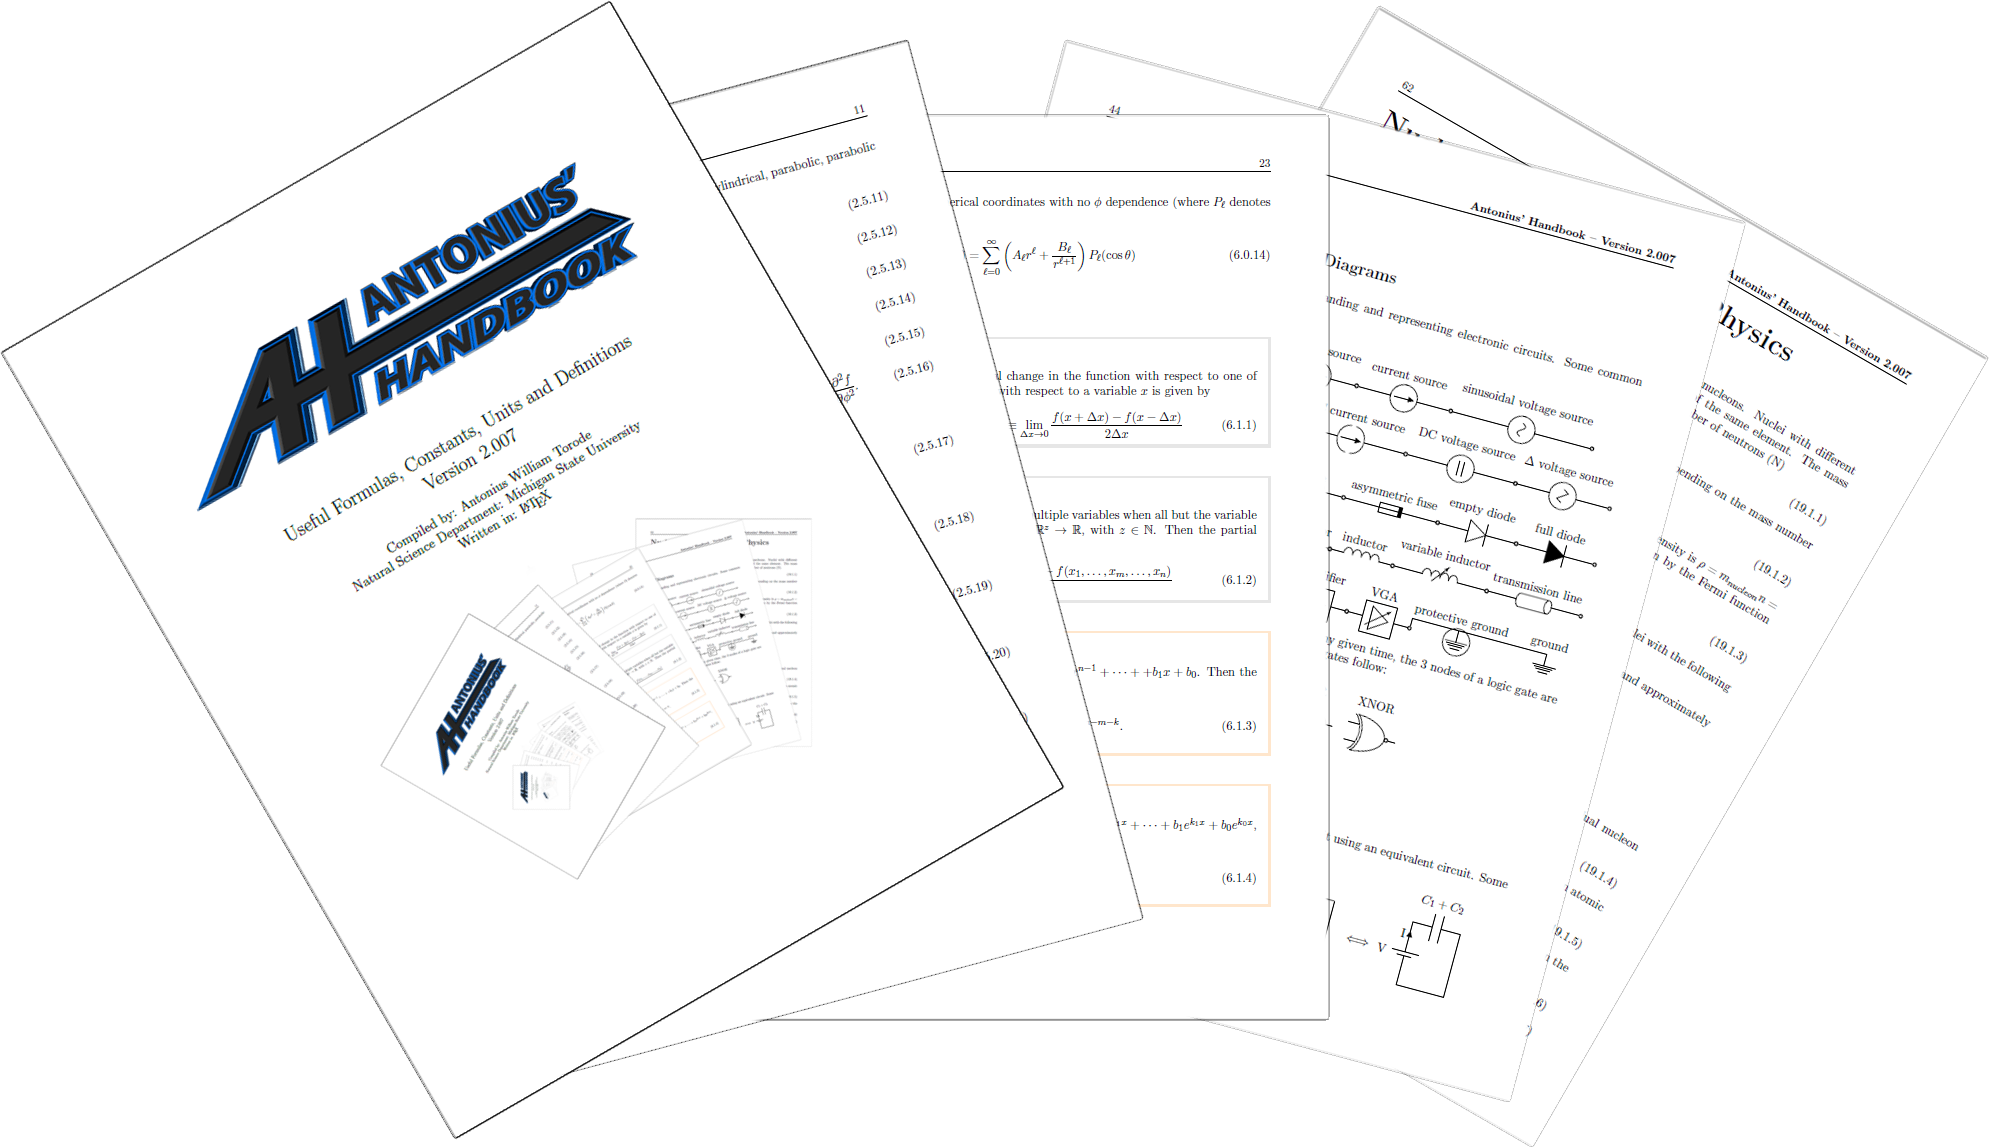
\includegraphics[scale=1.6]{./Images/Covers/background_tunnel.png}
\end{center}

%Copywrite page
\pagestyle{empty}
%% copyrightpage
\begingroup
\footnotesize
\parindent 0pt
\parskip \baselineskip
\textcopyright{} 2025 Antonius Torode \\
All rights reserved.

This work may be distributed and/or modified under the conditions of Antonius’ General Purpose License (AGPL).

The original maintainer of this work is: Antonius Torode.

The current maintainer of this work is: Antonius Torode.


Chief Editor: Antonius Torode

%\hfill\begin{minipage}{\textwidth-1cm}Other contributors:\end{minipage}

Published by Antonius Torode. 

Hosted at: https://torodean.github.io/

Github Repository: https://github.com/torodean/Antonius-Compendium

%\begin{center}
%\begin{tabular}{ll}
%First Personal Release (Version 0.000): & January 2016 \\
%First Public Release (Version 1.000): &  July 2016 \\
%Most Current Revision Date (Version \Version): & \today 
%\end{tabular}
%\end{center}

\vfill

Torode, A.\\
\hspace*{1em} Antonius' Compendium. \\
\hspace*{2em} Applied Research Laboratories -- \\
\hspace*{2em} \today \\
\hspace*{2em} Volume II. \\
\hspace*{2em} Version: \Version



\endgroup
\clearpage

%Preface page
\begin{center}
	\textbf{Preface}
\end{center}

This document is a compilation of ideas, scratch work, derivations, useful formulas, definitions, constants, and general information used for my own studies as a reference while furthering self education. These are my notes. It's purpose is to provide a complete 'compendium' per say of various ideas used often. All the material in this document was either directly copied from one of the references listed at the end or derived from scratch. On occasion \textit{typos may exist} due to human error but will be corrected when discovered.
	
The version number is updated every time the document is distributed, printed for distribution, or a major update is added. This ensures that there is no two copies with different information and similar version numbers. The latest update date is automatically set to the current date each time the document is edited. Please refrain from distributing this handbook without permission from the original author/compiler. This book is formatted for printing.

\begin{center}
	\textbf{Topics Covered In This Book}
\end{center}

\begin{multicols}{2}
\begin{itemize}
	\item Machine Learning
	\item Artificial Intelligence
	\item Modeling
	\item Psychology
\end{itemize} 
\end{multicols}

The information in this book is in no way limited to the topics listed above. They serve as a simple guideline to what you will find within this document. For more information about this book or details about how to obtain your own copy please visit:
\begin{center}
	https://torodean.github.io/
\end{center}

\begin{quotation}
``Scientific theories deal with concepts, not with reality. All theoretical results are derived from certain axioms by deductive logic. In physical sciences the theories are so formulated as to correspond in some useful sense to the real world, whatever that may mean. However, this correspondence is approximate, and the physical justification of all theoretical conclusions is based on some form of inductive reasoning.'' - Athanasios Papoulis (Probability, Random Variables, and Stochastic Processes book)
\end{quotation}

\begin{center}
	\textbf{Disclaimer}
\end{center}

This book contains formulas, definitions, and theorems that by nature are very precise. Due to this, some of the material in this book was taken directly from other sources such as but not limited to Wolfram Mathworld. This is only such in cases where a change in wording could cause ambiguities or loss of information quality.  Following this, all sources used are listed in the references section and cited when used.


%Begins blank page.
\thispagestyle{empty}
\newpage
\vspace*{\stretch{1}}
\begin{center}
	\textit{This page intentionally left blank.\\ (Yes, this is a contradiction.)}
\end{center}
\vspace*{\stretch{1}}

%Begins table of contents
\tableofcontents


%Begin the mainmatter.
\setlength{\parindent}{0pt}
\mainmatter
\pagestyle{fancy}
\include{./Chapters/Constants}

\newpage
\chapter{Statistics and Probability}
\thispagestyle{fancy}

\keyword{Probability} is a fundamental concept in mathematics and statistics that measures the likelihood of an event occurring. It is represented as a value between 0 and 1, where 0 indicates the event is impossible, 1 denotes certainty, and values between 0 and 1 represent various degrees of likelihood. In simple terms, probability quantifies how probable or likely it is for an event to happen based on the total number of possible outcomes. It helps us make informed decisions, predict outcomes, and understand uncertainty in various real-world scenarios, such as games of chance, weather forecasts, and medical diagnoses. To understand probability on a mathematical level, some definitions of terminology is needed.

A \keyword{state} (or outcome) is particular condition that something is in at a specific time. A \keyword{system} is an activity, experiment, process, or model with states or outcomes that are typically subject to uncertainty. A \keyword{sample space} of an system is the set of all possible states of a system. An \keyword{event} (also may be referred to as a trial or measurement) is any subset or collection of states contained in the sample space of a system. An event is a \keyword{simple event} if it consists of exactly one state and a \keyword{compound event} if it consistst of more than one state.

\begin{defn}[Probability]{Probability}
An \keyword{probability} $p$ can be defined as the asymptotic frequency of a system in the state $s$ ($s \in \Omega$, where $\Omega$ is the sample space of the system) by the total number of occurrences of that state $N_s$ in the limit of an infinite number of events $N$.
    \begin{align}
        p(s) = \lim_{N\rightarrow\infty}\frac{N_s}{N} \\
	p(s) \in [0,1] \forall s \in \Omega
    \end{align}
For a system with $n$ states, the total probabilities of all states must normalize to one.
    \begin{align}
        \sum_{i=0}^{n}p(i) = \sum_{s \in \Omega}p(i) = \lim_{N\rightarrow\infty}\frac{1}{N}\sum_{i=0}^{n}N_i = 1
    \end{align}
A \keyword{Bayesian probability} is defined as a person's knowledge of the outcome of a trial, based on the evidence at their disposal - often accompanied by an associated error. A \keyword{model probability} is an assumption or guess for the probability given the possibility of an infinite number of trials.
\end{defn}

Some more useful concepts for modeling a system are the mean (average) and standard deviation. 

\begin{defn}[Mean \label{Mean Definition}]
	If $x_1, ..., x_N$ denotes N separate measurements of one quantity $x$, then we define the mean (or average) $\braket{x}$ as
	\begin{align}
		\braket{x} = \frac{1}{N}\sum_{i=1}^{N}x_i \label{mean equation}
	\end{align}
\end{defn}

\begin{defn}[Standard Deviation \label{Standard Deviation Definition}]
	If $x_1, ..., x_N$ denotes N separate measurements of one quantity $x$, then we define the standard deviation $\sigma_x$ as
	\begin{align}
		\sigma_x = \sqrt{\frac{1}{N-1}\sum_{i}(x_i-\braket{x})^2}
	\end{align}
\end{defn}

When dealing with \keyword{Bayesian probability}, there is typically an uncertainty associated with the measurements or functions.

\begin{defn}[Mean \label{Mean Definition}]
	Suppose $x_0, ..., x_N$ denotes N separate measurements with associated uncertainties $\delta x_0, ..., \delta x_N$. If the measured values are used to compute some function $q(x_0, ..., x_N)$ and the uncertainties in $x_0, ..., x_N$ are independent and random, then the uncertainty in $q$ is
	\begin{align}
		\delta q = \sqrt{\sum_{i=0}^{N}\bigg(\frac{\delta q}{\delta x_i} \delta x_i\bigg)^2}.
	\end{align}
 It will always be true that 
 	\begin{align}
		\delta q \leq \sum_{i=0}^{N}\abs{\frac{\delta q}{\delta x_i}} \delta x_i.
	\end{align}
\end{defn}

\begin{defn}[Uncertainty \label{Uncertainty}]
	If $x_1, ..., x_N$ denotes N separate measurements of one quantity $x$, then we define the standard deviation $\sigma_x$ as
	\begin{align}
		\sigma_x = \sqrt{\frac{1}{N-1}\sum_{i}(x_i-\braket{x})^2}
	\end{align}
\end{defn}



\unchapter{Resources}

%Begin the backmatter.
\backmatter
{\footnotesize
\begin{thebibliography}{99}
%	\bibitem{bib:Modern_Physics} Bauer, W., and Gary D. Westfall. University Physics with Modern Physics. 2nd ed. Vol. 2. New York, NY: McGraw-Hill Companies, 2014. Print. 	
%	
%	\bibitem{bib:Methods_Of_Theoretical} Boas, Mary L. Mathematical Methods in the Physical Sciences. 3rd ed. New York: John Wiley \& Sons, 1984. Print. 
%	
%	\bibitem{bib:Planets_and_telescopes} Brown, Edward, comp. ``Planets And Telescopes." (2015): n. pag. Print. Michigan State University Department of Astronomy and Physics
%	
%	\bibitem{bib:AST304} Brown, Edward, comp. Astronomy 304 class handouts (2015): n. pag. Print. Michigan State University Department of Astronomy and Physics
%	
%	\bibitem{bib:StellarAstrophysics} Brown, Edward, comp. ``Stellar Astrophysics." (2015): n. pag. Print. Michigan State University Department of Astronomy and Physics
%	
%	\bibitem{bib:dictionary} http://www.dictionary.com
%	
%	\bibitem{bib:Griffiths} Griffiths, David J. Introduction to Electrodynamics. 4th ed. N.p.: Pearson India Education Services Pvt, 2015. Print. 
%	
%	\bibitem{Demtroder} Demtr\"{o}der, Wolfgang. Atoms, Molecules and Photons an Introduction to Atomic, Molecular, and Quantum-Physics: with 677 Figures and 42 Tables. Springer, 2010. 
%	
%	\bibitem{bib:Griffiths_QM}  Griffiths, David J. Introduction to Quantum Mechanics. 2nd ed. Harlow: Pearson, 2014. Print. 
%	
%	\bibitem{bib:PDE book} Haberman, R. "Applied Partial Differential Equations: with Fourier series and Boundary Value Problems." 4th ed. Upper Saddle River, New Jersey. 2004. Print.
%	
%	\bibitem{bib:PeriodicTable} Helmenstine, Todd. Periodic Table of the Elements. sciencenotes.org. 2015.
%	
%	\bibitem{Abstract Algebra} Judson T. W. "Abstract Algebra: Theory and Applications." Stephen F. Austin State University. August 5, 2017.
%	
%	\bibitem{bib:Linnemann} Linnemann, Jim, Dr. Modern Physics Lecture Notes. 2016. PHY 215 lecture notes. Department of Physics and Astronomy, Michigan State University. 
%	
%	\bibitem{bib:AbstractNotes} Meierfrankenfeld, Ulrich. MTH 310 Lecture Notes Based on Hungerford, Abstract Algebra. N.p.: Department of Mathematics, Michigan State U, 2015. Print. 
%	
%	\bibitem{electronics} Plonus, Martin. Electronics and Communications for Scientists and Engineers. San Diego: Academic, 2001. Print. 
%	
%	\bibitem{bib:ReitzEMTheory} Reitz, John Richard. Foundations of Electromagnetic Theory. 4th ed. N.p.: Addison-Wesley, 1992. Print. 
%	
%	\bibitem{bib:Kittel_ThermalPhysics}  Kittel, Charles, and Herbert Kroemer. Thermal Physics. San Francisco: W.H. Freeman, 1980. Print.
%	
%	\bibitem{Nazarewicz_PHY802} Nazarewicz, Witek. "MSU PHY802 Lecture Slides." Survey of Nuclear Physics 802/492 Spring 2017. Michigan State University, n.d. Web. 31 Mar. 2017. 
%	
%	\bibitem{Elementary Analysis} Ross, Kenneth A. Elementary Analysis: The Theory of Calculus $2^{\textrm{nd}}$ edition. 
%	
%	\bibitem{bib:Foundations_Of_Astrophysics} Ryden, Barbara Sue., and Bradley M. Peterson. Foundations of Astrophysics. San Francisco: Addison-Wesley, 2010. Print. 
%	
%	\bibitem{bib:elementTable} ``Table of Isotopic Masses and Natural Abundances." (n.d.): n. pag. NC State University. Web. ``https://www.ncsu.edu/chemistry/msf/pdf/IsotopicMass\_NaturalAbundance.pdf". 
%	
%	\bibitem{bib:Classical_Mechanics} Taylor, John R. Classical Mechanics. Sausalito, CA: U Science, 2005. Print. 
%	
%	\bibitem{bib:WolfrmAlpha} ``Wolfram$|$Alpha: Computational Knowledge Engine." N.p., n.d. Web. 2016 x
%	
%	\bibitem{bib:Wolfram} ``Wolfram MathWorld: The Web's Most Extensive Mathematics Resource." Wolfram MathWorld. N.p., n.d. Web. 
%	
%	\bibitem{DiffEQ} Zee, Dennis G. A first Course in Differential Equations with Modeling Applications." Edition 10. Book.
\end{thebibliography}
}

\printindex

\end{document}